% ===================== PARTE 3: RENDIMIENTO (diapositivas 31-46) =====================
\parte{Rendimiento}{Rendimiento: la figura 5, frente al paper}
  {Los binarios oficiales en el Core Ultra 9, escenario por escenario: qué se repite, qué no, y qué lo explica.}{s31}

\begin{frame}{El paper: cuatro Xeon, hasta 216 hilos}
  \fuente{paper\_fig5.csv, extraído del PDF vectorial con herramientas/extraer\_fig5.py}
  \centering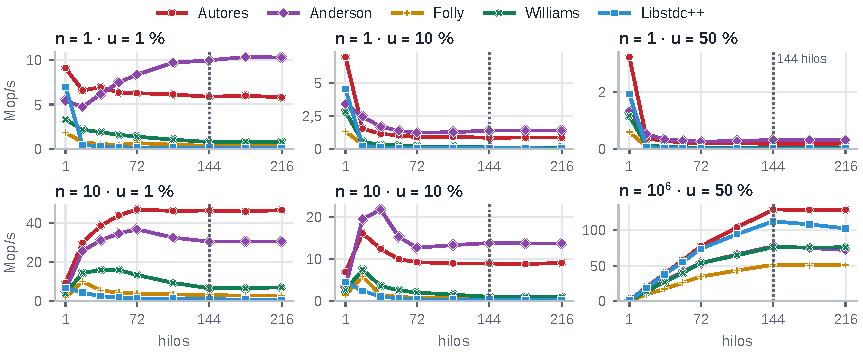
\includegraphics[width=\linewidth]{figuras/s32}
  \nota{s32}
\end{frame}

\begin{frame}{La réplica: Core Ultra 9, binarios oficiales, con Docker}
  \fuente{docker/rendimiento.csv; mediana de 5 rondas de 2\,s; la sombra va de la peor ronda a la mejor}
  \centering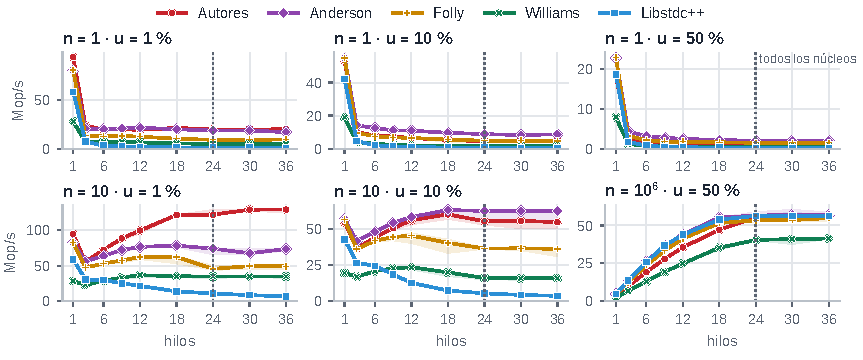
\includegraphics[width=\linewidth]{figuras/s33}
  \nota{s33}
\end{frame}

\begin{frame}{De 1 a 3 hilos casi todo se desploma, salvo con un millón de pilas}
  \fuente{docker/rendimiento.csv, Autores, mediana de 5 rondas}
  \begin{columns}[T]
    \column{0.47\textwidth}\small\renewcommand{\arraystretch}{1.15}
    \begin{tabular}{@{}lrrr@{}}
      \toprule
      \textbf{Autores} (Mop/s) & \textbf{1 hilo} & \textbf{3 hilos} & \textbf{Cambio}\\
      \midrule
      $n = 1$ · $u = 1$\,\% & 94,2 & 23,7 & $-75$\,\%\\
      $n = 1$ · $u = 10$\,\% & 53,4 & 10,1 & $-81$\,\%\\
      $n = 1$ · $u = 50$\,\% & 18,3 & 2,5 & $-86$\,\%\\
      $n = 10$ · $u = 1$\,\% & 94,6 & 55,5 & $-41$\,\%\\
      $n = 10$ · $u = 10$\,\% & 54,7 & 36,6 & $-33$\,\%\\
      $n = \pot{6}$ · $u = 50$\,\% & 3,3 & 9,9 & \textcolor{verde}{\textbf{+200\,\%}}\\
      \bottomrule
    \end{tabular}
    \column{0.49\textwidth}
    \porque{contención por una línea de caché}{Los datos viajan entre núcleos en líneas de 64 bytes, y para escribir en una línea un núcleo tiene que tenerla en exclusiva. Si todos escriben en la misma, la línea pasa de mano en mano: el trabajo dura un instante y lo que cuesta es el viaje. Más hilos no aceleran nada: añaden viajes.\par\smallskip
    Con un millón de pilas, dos hilos casi nunca tocan la misma línea, y el rendimiento sube con los hilos, como uno esperaría.}
  \end{columns}
  \vfill
  \caja{Esta es la teoría que explica casi todas las gráficas: lo caro no es calcular, es \textbf{mover la línea compartida}.}
  \nota{s34}
\end{frame}

\begin{frame}{El marcador con toda la máquina: coincide quién gana en 4 de 6}
  \fuente{docker/rendimiento.csv y paper\_fig5.csv; EXPLICACION.md, Parte 6.1}
  \footnotesize\renewcommand{\arraystretch}{1.18}
  \begin{tabularx}{\linewidth}{@{}p{0.19\linewidth}p{0.2\linewidth}p{0.16\linewidth}Xp{0.13\linewidth}@{}}
    \toprule
    \textbf{Escenario} & \textbf{En palabras} & \textbf{Paper, 144 hilos} & \textbf{Réplica, 24 hilos} & \textbf{¿Coincide?}\\
    \midrule
    $n = 1$ · $u = 1$\,\% & 1 pila, casi solo lecturas & Anderson (1,70\por) & Autores, por poco (Anderson 0,94\por) & \textcolor{rojo}{\textbf{No}}\\
    $n = 1$ · $u = 10$\,\% & 1 pila, algunas escrituras & Anderson (1,66\por) & Anderson (1,99\por) & \textcolor{verde}{\textbf{Sí}}\\
    $n = 1$ · $u = 50$\,\% & 1 pila, muchas escrituras & Anderson (1,82\por) & Anderson (1,87\por) & \textcolor{verde}{\textbf{Sí}}\\
    $n = 10$ · $u = 1$\,\% & 10 pilas, casi solo lecturas & Autores (Anderson 0,66\por) & Autores (Anderson 0,61\por) & \textcolor{verde}{\textbf{Sí}}, casi igual\\
    $n = 10$ · $u = 10$\,\% & 10 pilas, algunas escrituras & Anderson (1,54\por) & Anderson (1,13\por) & \textcolor{verde}{\textbf{Sí}}, por menos\\
    $n = \pot{6}$ · $u = 50$\,\% & un millón de pilas & Autores & Empate a cuatro, unos 55\,Mop/s & \textcolor{rojo}{\textbf{No}}\\
    \bottomrule
  \end{tabularx}
  \vfill
  \caja{El mejor caso de Autores se reproduce casi exacto: con $n = 10$ y $u = 1$\,\%, Autores 122\,Mop/s, Anderson 74, Folly 46, Williams 35 y Libstdc++ 11.}
  \nota{s35}
\end{frame}

\begin{frame}{Cada rival respecto a Autores: paper frente a réplica}
  \fuente{paper\_fig5.csv, docker y nativo\_oficial/rendimiento.csv; 144 hilos en el paper, 24 en la réplica}
  \centering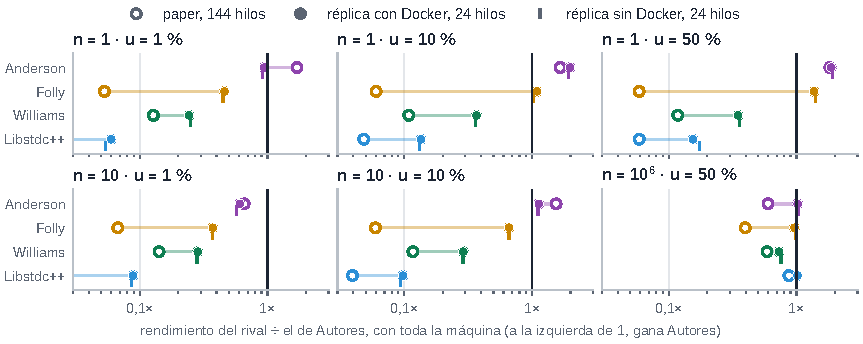
\includegraphics[width=\linewidth]{figuras/s36}
  \nota{s36}
\end{frame}

\begin{frame}{Lo que se repite, y la teoría que lo explica}
  \fuente{docker/rendimiento.csv; EXPLICACION.md, Partes 3 y 6.1}
  \begin{columns}[T]
    \column{0.48\textwidth}\footnotesize
    {\bfseries\alg{cLibs}{Libstdc++ se hunde al crecer los hilos}}\par\smallskip
    De 58,5 a 1,2\,Mop/s con $n = 1$ y $u = 1$\,\%: unas 49 veces menos. En el paper, de 7 a 0,11: unas 64 veces.\par
    \emph{Por qué:} un candado forma una cola. Cada lectura escribe dos veces en la línea más disputada, y quien no entra se queda dando vueltas.
    \par\medskip
    {\bfseries\alg{cWilliams}{Williams queda por debajo en los 6 escenarios}}\par\smallskip
    Entre 0,24\por{} y 0,73\por{} de Autores.\par
    \emph{Por qué:} cada lectura necesita dos bucles de CAS de 16 bytes (\texttt{cmpxchg16b}) que pueden fallar y repetirse. Autores hace una sola resta que nunca falla.
    \column{0.48\textwidth}\footnotesize
    {\bfseries\alg{cAnderson}{Anderson gana con escrituras sobre pocas pilas}}\par\smallskip
    1,87\por{} a 1,99\por{} con $n = 1$ y $u \ge 10$\,\%.\par
    \emph{Por qué:} en Autores cada lectura modifica la palabra compartida, así que el CAS de quien escribe falla por culpa de los lectores. En Anderson leer no escribe en esa palabra.
    \par\medskip
    {\bfseries\alg{cAutores}{Autores brilla con lecturas y algo de reparto}}\par\smallskip
    $n = 10$, $u = 1$\,\%: 122\,Mop/s, 1,65\por{} Anderson.\par
    \emph{Por qué:} con pocas escrituras casi no hay CAS que fallen, y su lectura es la más barata: una instrucción, sin bucle.
  \end{columns}
  \vfill
  \caja{La diferencia que lo explica casi todo es una sola instrucción: \texttt{fetch\_sub} no puede fallar; un CAS sí, y con contención falla una y otra vez.}
  \nota{s37}
\end{frame}

\begin{frame}{Por qué Anderson gana con escrituras sobre una sola pila}
  \fuente{EXPLICACION.md, Partes 3.5, 3.6 y 3.7}
  \centering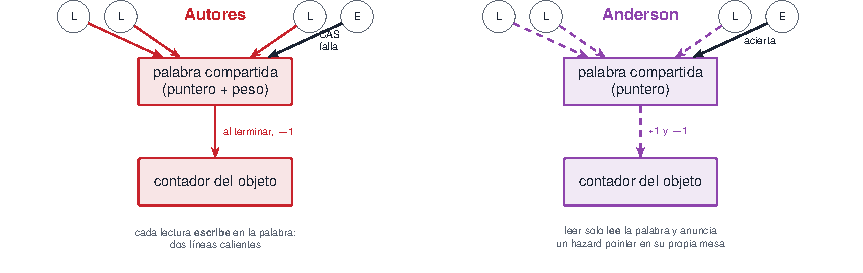
\includegraphics[width=\linewidth]{figuras/s38}
  \vfill\raggedright
  \caja{Precio de Anderson: no puede liberar en el acto. Guarda los bloques de control en una caja de pendientes (\hyperlink{parte8}{parte 8}) y paga picos de latencia al vaciarla (\hyperlink{parte7}{parte 7}).}
  \nota{s38}
\end{frame}

\begin{frame}{Lo que no se repite (1): Folly rinde muchísimo mejor que en el paper}
  \fuente{docker, nativo\_oficial/rendimiento.csv y paridad.csv; EXPLICACION.md, Parte 6.1}
  \begin{columns}[T]
    \column{0.5\textwidth}\small\renewcommand{\arraystretch}{1.2}
    \begin{tabular}{@{}lr@{}}
      \toprule
      \textbf{Folly ÷ Autores, con contención} &\\
      \midrule
      Paper, 144 hilos & 0,05\por{} a 0,07\por\\
      Réplica con Docker, 24 hilos & 0,37\por{} a 1,37\por\\
      Réplica sin Docker, 24 hilos & 0,37\por{} a 1,40\por\\
      Receta exacta, 10\,s \por{} 7 & 0,36\por{} a 1,26\por\\
      \bottomrule
    \end{tabular}
    \par\medskip\footnotesize
    Con $n = 1$ y $u = 50$\,\% Folly incluso \textbf{gana}: 1,47 frente a 1,07\,Mop/s, sin que los rangos de las rondas se toquen.
    \column{0.46\textwidth}
    \caja{\textbf{Descartados:} ni Docker ni el recorte de duración explican la diferencia. Se midió sin Docker y con la receta exacta del paper, y sale lo mismo.}
    \par\medskip
    \aviso{La explicación fácil, «el paper tiene 4 sockets y aquí hay uno», no se sostiene. La siguiente diapositiva muestra por qué.}
  \end{columns}
  \nota{s39}
\end{frame}

\begin{frame}{La brecha de Folly ya existe con un solo hilo}
  \fuente{paper\_fig5.csv y docker/rendimiento.csv, con 1 hilo; EXPLICACION.md, Parte 6.1}
  \centering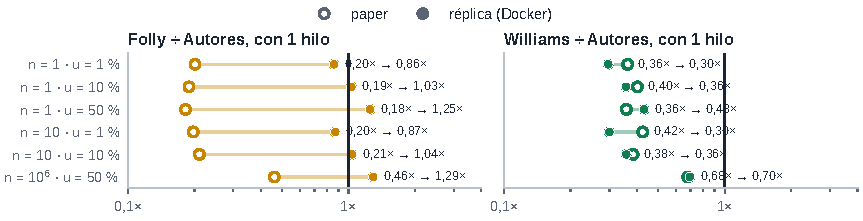
\includegraphics[width=\linewidth]{figuras/s40}
  \vfill\raggedright
  \porque{por qué un hilo descarta la contención}{Con un hilo no hay pelea ni líneas que viajen entre núcleos. Si la relación Folly ÷ Autores ya es de 3 a 7 veces peor en el paper que aquí, la causa no es la contención ni la distancia; Williams, en cambio, coincide. Y en la figura 6 del paper, el \texttt{load} de Folly sin contención tarda 24\,ns, como Autores (23\,ns). \textbf{Pregunta abierta:} algo de la máquina de la figura 5, o de cómo se midió allí, penaliza a Folly.}
  \nota{s40}
\end{frame}

\begin{frame}{Lo que no se repite (2): con una pila y pocas escrituras, Anderson no llega a adelantar}
  \fuente{paper\_fig5.csv y docker/rendimiento.csv; EXPLICACION.md, Parte 6.1}
  \begin{columns}[T]
    \column{0.5\textwidth}\footnotesize\renewcommand{\arraystretch}{1.18}
    \begin{tabular}{@{}lll@{}}
      \toprule
      \textbf{Anderson ÷ Autores} & \textbf{Paper} & \textbf{Réplica}\\
      \midrule
      18 hilos & 0,72\por & 0,94\por\\
      36 hilos & 0,89\por & ---\\
      54 hilos o más & > 1: adelanta & no hay núcleos\\
      24 hilos (toda la máquina) & --- & 0,94\por\\
      \bottomrule
    \end{tabular}
    \par\smallskip{\scriptsize $n = 1$ · $u = 1$\,\%.}
    \column{0.46\textwidth}
    \caja{En el paper, Anderson solo adelanta a Autores a partir de 54 hilos. Esta máquina tiene 24 núcleos: no llega a la zona donde ocurre el cruce. A igual número de hilos, los dos resultados no están lejos.}
  \end{columns}
  \vfill
  \porque{dos líneas calientes frente a una}{Con una sola pila y muchos lectores, Autores tiene dos líneas disputadas, la palabra y el contador del objeto; Anderson solo una, el contador. Con suficientes hilos, esa segunda línea acaba pesando más que la lectura barata de Autores. Aquí no hay hilos suficientes para verlo.}
  \nota{s41}
\end{frame}

\begin{frame}{Lo que no se repite (3): con un millón de pilas, cuatro algoritmos empatan}
  \fuente{docker/rendimiento.csv, 24 hilos; paper\_fig5.csv, 144 hilos}
  \begin{columns}[T]
    \column{0.42\textwidth}\small\renewcommand{\arraystretch}{1.15}
    \begin{tabular}{@{}lrr@{}}
      \toprule
      $n = \pot{6}$ · $u = 50$\,\% & \textbf{Réplica} & \textbf{Paper}\\
      \midrule
      \alg{cAnderson}{Anderson} & 56,5 & ---\\
      \alg{cLibs}{Libstdc++} & 56,3 & ---\\
      \alg{cAutores}{Autores} & 55,4 & 129\\
      \alg{cFolly}{Folly} & 53,4 & ---\\
      \alg{cWilliams}{Williams} & 40,4 & ---\\
      \bottomrule
    \end{tabular}
    \par\smallskip{\scriptsize Mop/s; en el paper, Autores lidera con claridad.}
    \column{0.54\textwidth}
    \caja{Que cuatro algoritmos tan distintos toquen el mismo techo sugiere que el límite no está en el algoritmo, sino en algo común a todos.}
    \par\medskip
    \porque{sospecha}{Con un millón de pilas, casi cada operación tiene que ir a la RAM. Este PC tiene un solo módulo de memoria, un solo canal; el paper tenía 4 chips, cada uno con su memoria.}
  \end{columns}
  \nota{s42}
\end{frame}

\begin{frame}{El techo era la RAM: lo dicen los contadores de la controladora de memoria}
  \fuente{memoria\_ram.csv (herramientas/medir\_memoria.py), binarios oficiales, $n = \pot{6}$, $u = 50$\,\%; 2 rondas}
  \centering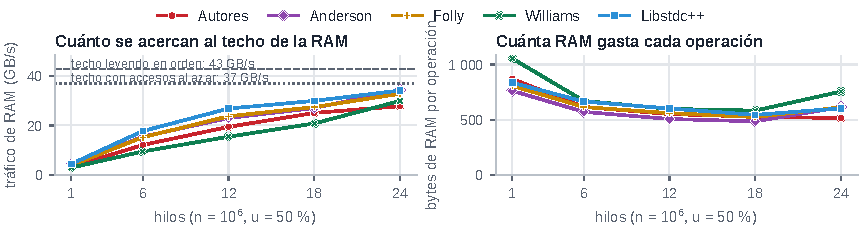
\includegraphics[width=\linewidth]{figuras/s43}
  \par\smallskip\footnotesize\renewcommand{\arraystretch}{1.12}
  \begin{tabular}{@{}l*{5}{p{0.13\linewidth}}@{}}
    \toprule
    \textbf{24 hilos} & \alg{cAnderson}{Anderson} & \alg{cLibs}{Libstdc++} & \alg{cFolly}{Folly} & \alg{cWilliams}{Williams} & \alg{cAutores}{Autores}\\
    \midrule
    \% del techo al azar & 93\,\% & 92\,\% & 89\,\% & 81\,\% & 75\,\%\\
    Bytes por operación & 615 & 603 & 613 & 755 & \textbf{515}\\
    \bottomrule
  \end{tabular}
  \nota{s43}
\end{frame}

\begin{frame}{Lo que dicen los contadores, y lo que no}
  \fuente{memoria\_ram.csv; EXPLICACION.md, Partes 6.1 y 8}
  \begin{columns}[T]
    \column{0.48\textwidth}
    {\color{verde}\bfseries Refuerza la explicación}\par\smallskip
    \begin{itemize}\footnotesize
      \item Anderson, Libstdc++ y Folly rozan el techo y casi dejan de crecer: Anderson pasa de 54,2 a 54,5\,Mop/s de 18 a 24 hilos, mientras su tráfico sube de 27 a 34\,GB/s.
      \item Con 36 hilos, ninguno pasa de 57\,Mop/s.
      \item Autores mueve entre un 15 y un 32\,\% menos bytes por operación.
    \end{itemize}
    \column{0.48\textwidth}
    {\color{rojo}\bfseries Pero no lo explica todo}\par\smallskip
    \begin{itemize}\footnotesize
      \item Autores rinde igual con solo el 75\,\% del techo: algo más lo frena, quizá la espera de cada acceso. No se midió.
      \item El techo al azar solo lee, y las pilas leen y escriben.
      \item La prueba definitiva sería repetirlo con \textbf{dos módulos de RAM}: si el rendimiento sube, queda demostrado.
    \end{itemize}
  \end{columns}
  \vfill
  \aviso{La primera versión de la medida casi nos engaña: miraba los últimos segundos, cuando el programa ya liberaba memoria, y dio 14\,GB/s. Lo delató que el tráfico no crecía con el rendimiento. La versión corregida mira solo la mitad central de cada ejecución.}
  \nota{s44}
\end{frame}

\begin{frame}{Por debajo del techo, Autores va por detrás con pocos hilos}
  \fuente{docker y nativo\_oficial/rendimiento.csv; memoria\_ram.csv; EXPLICACION.md, Parte 6.1}
  \begin{columns}[T]
    \column{0.54\textwidth}\footnotesize\renewcommand{\arraystretch}{1.18}
    \begin{tabular}{@{}lrrr@{}}
      \toprule
      $n = \pot{6}$ · $u = 50$\,\% & \textbf{1 hilo} & \textbf{12 hilos} & \textbf{Paper, 1 hilo}\\
      \midrule
      Anderson ÷ Autores & 1,46\por & 1,24\por & 1,03\por\\
      Libstdc++ ÷ Autores & 1,44\por & 1,24\por & 0,87\por\\
      \midrule
      Sin Docker: Anderson & 1,33\por & 1,19\por &\\
      Sin Docker: Libstdc++ & 1,40\por & 1,19\por &\\
      \bottomrule
    \end{tabular}
    \column{0.42\textwidth}
    \caja{Mover más bytes no lo explica: con 6 hilos, Autores mueve 617 bytes por operación, Anderson 572 y Libstdc++ 666. Libstdc++ mueve más que Autores y aun así va 1,38\por{} más rápido.}
    \par\medskip
    \aviso{\textbf{Pregunta abierta.} No es Docker: sin Docker se repite. Afecta a la fila 5 del veredicto.}
  \end{columns}
  \nota{s45}
\end{frame}

\begin{frame}{¿Se parece el orden? La $\tau$ de Kendall, escenario por escenario}
  \fuente{resultados/david-ultra9-285/tablas.md, «Rendimiento: paper (144 hilos) frente a réplica (24 hilos)»}
  \begin{columns}[T]
    \column{0.36\textwidth}\small\renewcommand{\arraystretch}{1.18}
    \begin{tabular}{@{}lr@{}}
      \toprule
      \textbf{Escenario} & \textbf{$\tau$ de Kendall}\\
      \midrule
      $n = 1$ · $u = 1$\,\% & +0,60\\
      $n = 1$ · $u = 10$\,\% & +0,60\\
      $n = 1$ · $u = 50$\,\% & +0,40\\
      $n = 10$ · $u = 1$\,\% & +0,80\\
      $n = 10$ · $u = 10$\,\% & +0,80\\
      $n = \pot{6}$ · $u = 50$\,\% & +0,20\\
      \bottomrule
    \end{tabular}
    \column{0.6\textwidth}
    \porque{la tau de Kendall}{Compara dos clasificaciones pareja a pareja: +1 es el mismo orden, 0 sin relación y $-1$ al revés. Con 5 algoritmos hay 10 parejas; +0,60 significa 8 de acuerdo y 2 en desacuerdo.}
    \par\medskip
    \caja{Siempre positiva: el orden siempre se parece. En los cinco primeros escenarios, casi todo el desacuerdo viene de Folly. El +0,20 final es el empate: el orden entre iguales no significa nada.}
  \end{columns}
  \nota{s46}
\end{frame}
